\documentclass{beamer}
\usetheme{CambridgeUS}

\usepackage{graphicx}
\usepackage{subcaption}
\usepackage{natbib}
\usepackage{booktabs}

\DeclareMathOperator*{\argmin}{argmin}

\title[GHSOM for Community Detection]{Growing Hierarchical Self Organizing Maps for Community Detection}
\author{David McDonald \and Shan He}
%\institute{University of Birmingham, \\ Birmingham, UK \\ B15 2TT}
\date{10th April 2017}

\begin{document}
	
	\begin{frame}
		\titlepage
	\end{frame}
	
	\begin{frame}{Recap}
		
		\begin{itemize}
			\item Using Growing Hierarchical Self Organising Maps to detect communities at multiple scales in complex networks. 
			\item Achieved very good NMI scores on synthetic hierarchical benchmarks.
			\item Was capable of good NMI scores on real world benchmarks, but finding a principled methodology of setting parameters was challenging.
		\end{itemize}
		
	\end{frame}
	
	\begin{frame}{Results on Synthetic Networks}
		\begin{figure}
			\centering
			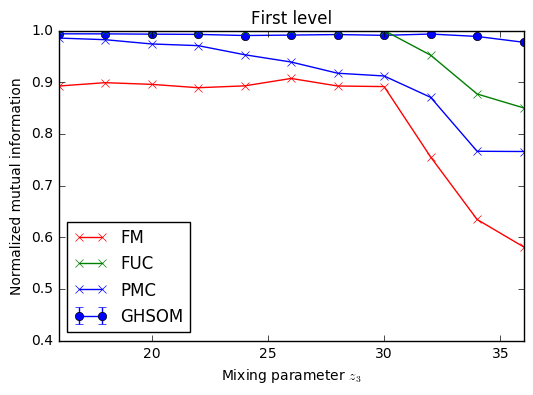
\includegraphics[scale=0.45]{first_level.png}
			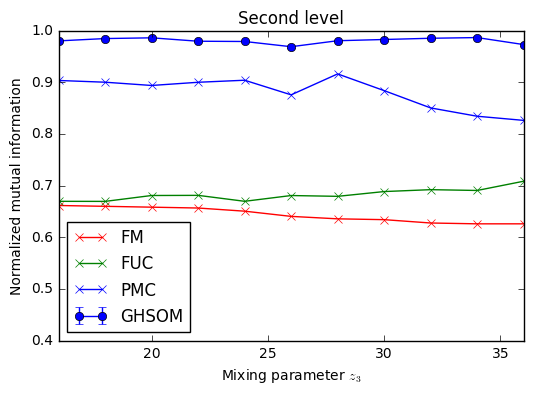
\includegraphics[scale=0.45]{second_level.png}
			\caption{Plot of mixing parameter $z_3$ against NMI score for both levels of community. 100 networks were generated with each mixing parameter. Results extracted without permission from \protect			\cite{yang2013hierarchical} (fig 4).}
			\label{synthetic_experiment}
		\end{figure}
	\end{frame}
	
	\begin{frame}{Results on Real World Networks}
		\begin{table}
			\centering
			\begin{tabular}{ c c c c c }
				\toprule
				\textbf{Algorithm} & \multicolumn{4}{c}{\textbf{Network (NMI Score)}}\\
				{} & Karate & Dolphin & Polbooks & Football \\ 
				\bottomrule
				\textbf{\#comms} & 2 & 4 & 3 & 12 \\
				\bottomrule 
				MCL & \textbf{1.000} & 0.424 & 0.515 & \textbf{0.935} \\ 
				FM & 0.693 & 0.509 & 0.531 & 0.757 \\ 
				%LP & 0.601 & 0.544 & 0.517 & 0.895 \\ 
				%Infomap & 0.699 & 0.566 & 0.537 & 0.924 \\ 
				FUC & 0.587 & \textbf{0.636} & \textbf{0.575} & 0.855 \\ 
				%MRW & 0.562 & 0.549 & 0.543 & 0.887 \\ 
				PMC & 0.837 & 0.620 & 0.574 & 0.887 \\ 
				\toprule
				GHSOM ($\epsilon_{sg}=0.6$) & 0.500 & 0.523 & 0.516 & 0.739 \\
				GHSOM ($\epsilon_{sg}=0.8$) & 0.733 & 0.575 & 0.547 & 0.528 \\
				\bottomrule
			\end{tabular}
			\caption{Table of NMI scores of GHSOM versus several algorithms in the literature. The best NMI score for each network is written in bold. Results for comparison algorithms are taken from \protect\cite{yang2013hierarchical} (table 2) without permission. }
			\label{real_world_experiment}
		\end{table}
	\end{frame}
	
	\begin{frame}{Bayesian Optimisation}
		\begin{table}
			\centering
			\begin{tabular}{l l l l l}
				\bottomrule
				\textbf{Parameter} & \multicolumn{4}{c}{\textbf{Network (NMI Score)}} \\
				{} & Karate & Dolphin & Polbook & Football \\
				\bottomrule
				\textbf{\#comms} & 2 & 4 & 3 & 12 \\
				\bottomrule 
				$\eta$ & 0.0001 & 0.879 & 0.999 & 0.0587 \\
%				$w$ & 0.943 & 0.0001 & 0.353 & 0.0663 \\
				$\sigma$ & 0.817 & 0.001 & 0.650 & 1.0 \\
				$\epsilon_{sg}$ & 0.988 & 0.558 & 1.0 &  0.451 \\
				$\epsilon_{en}$ & 1.0 & 0.3 & 0.393 & 0.3 \\
				\bottomrule
				\textbf{\#comms det.} & 2 & 4 & 2 & 11 \\
				\textbf{NMI score} & \textbf{1.0} & \textbf{0.640} & \textbf{0.688} & 0.874 \\
				\bottomrule
			\end{tabular}
			\caption{Spearmint optimized parameter settings and NMI scores for real world networks (to 3 s.f.). Spearmint provided by \protect\cite{snoek2012practical}.}
			\label{bayes}
		\end{table}	
	\end{frame}
	
	\begin{frame}{Current Research: Topological Functional Similarity Neighbouring Communities}
		Do neighbouring communities cooperate?
		\begin{figure}
			\centering
			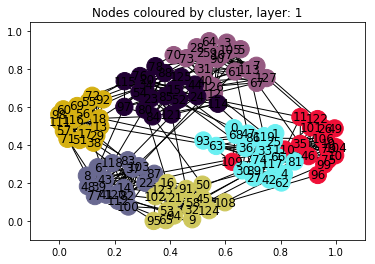
\includegraphics[scale=0.4]{figure2_network.png}
			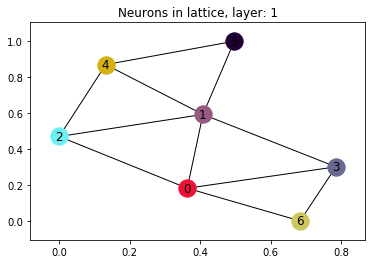
\includegraphics[scale=0.4]{figure2_map.png}
			\caption{Visualisation of simple generated network and resulting map. Nodes are coloured in the network by the neuron in the map that they are assigned to.}
			\label{colouring}
		\end{figure}
	\end{frame}
	
	\begin{frame}{A Little Background: The Gene Ontology (GO)}
		
		\begin{itemize}
			\item A controlled vocabulary to share information about all genes across all \textit{eukaryotes} (organisms with cells containing a nucleus) (\cite{ashburner2000gene}).
			\item Represented as three directed acyclic graphs (DAGs) corresponding to the three ontologies: Biological Process (BP), Molecular Function (MF), and Cellular Component (CC).
			\item Nodes on the graph are GO terms and edges are relations.
			\item Genes are annotated with GO terms using annotation databases.
			\item All annotations obey the true path rule: if a gene is annotated with a term then it is automatically annotated with all of that term's ancestors.  
		\end{itemize}
		
	\end{frame}
	
	\begin{frame}
		
		\begin{figure}
			\centering
			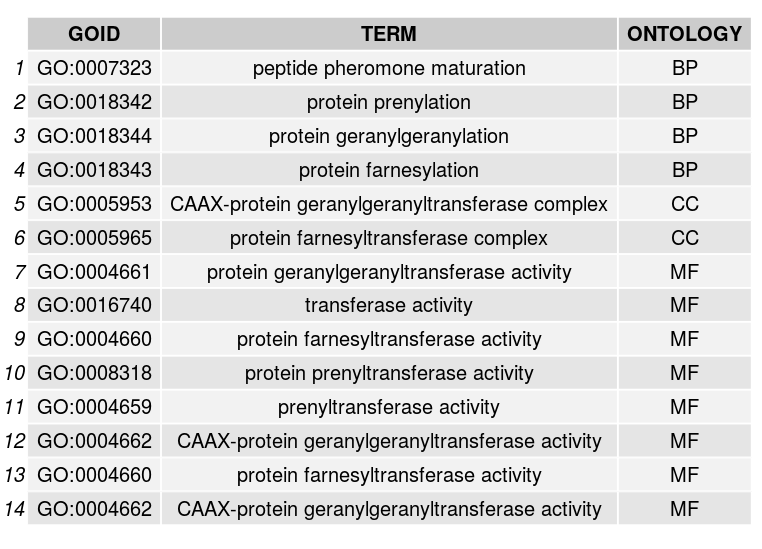
\includegraphics[scale=0.4]{go_terms_YKL019W.png}
			\caption{All GO terms annotated to the gene with ORF identifier YKL019W in the org.Sc.sgd.db annotation database. YKL019W is automatically annotated with the parents of all these terms due to the true path rule of GO.}
			\label{all_go_YKL019W}
		\end{figure}
		
	\end{frame}
	
	\begin{frame}
		\begin{figure}
			\centering
			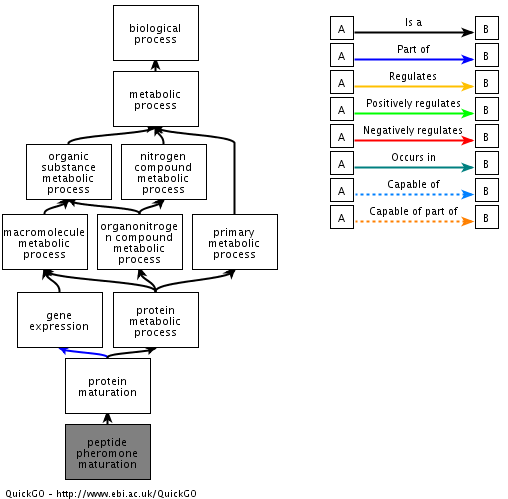
\includegraphics[scale=0.4]{GO:0007323.png}
			\caption{All ancestors of the GO term GO:0007313 \textit{peptide pheromone maturation} in the BP ontology.}
		\end{figure}
	\end{frame}
	
	\begin{frame}{Experiments on Saccharomyces Cerevisiae}
		\begin{itemize}
			\item Experimented on two \textit{Saccharomyces Cerevisiae} (budding yeast) co-expression networks. 
			\item Found largest fully connected component in each network and embedded using MDS, based on shortest path between each pair of genes in the network.
		\end{itemize}
		\begin{table}
			\centering
			\begin{tabular}{c c c}
				\toprule
				\textbf{Network name} & \textbf{Number of Nodes} & \textbf{Number of Edges} \\ \bottomrule
				Uetz Screen & 263 & 292 \\
				Y2H Union & 1647 & 2682 \\ \bottomrule
			\end{tabular}
			\caption{Topology information for the two Saccharomyces Cerevisiae networks. Datasets available from \protect\cite{uetz,union}.}
			\label{yeast_networks}
		\end{table}
	\end{frame}
	
	\begin{frame}{Method}
		\begin{itemize}
			\item Use GHSOM to partition network into set of communities.
			\item For each community, determine the set of enriched GO terms using a 2x2 contingency table and Fisher's exact test.
			\item Select terms based on p-value 0.05.	
		\end{itemize}
		
		\begin{figure}
			\centering
			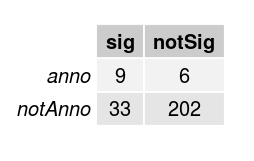
\includegraphics[scale=0.7]{contingency_table.png}
			\caption{An example contingency table for the go term: GO:0006914 \textit{autophagy} (p-value=0.000111024375808973).}
		\end{figure}
		
	\end{frame}
	
	\begin{frame}{Similarity Measures}
		Two similarity measures used so far. Both very prominent in the literature.
		
		\begin{itemize}
			\item \cite{resnik1999semantic}
			\begin{itemize}
				\item Originally used on words.
				\item Assigns measure of \textit{information content} based on number of offspring.
				\item Lower terms in the DAG contain more information.
				\item The similarity of two terms is the greatest information content of their common ancestors.
				\item ``Resnik's measure correlates well with gene expression'' (\cite{sevilla2005correlation}).
			\end{itemize}
			\item \cite{wang2007new}
			\begin{itemize}
				\item Based on topology of DAG.
				\item Weightings are assigned to each relation.
				\item Recursively assign semantic value to each term in the DAG induced from a given term, by using edge weights.
				\item Semantic similarity of two terms proportional to the number of terms in both DAGs.
			\end{itemize}
		\end{itemize}

	\end{frame}
	
	\begin{frame}{Results}
		
		\begin{figure}
			\centering
			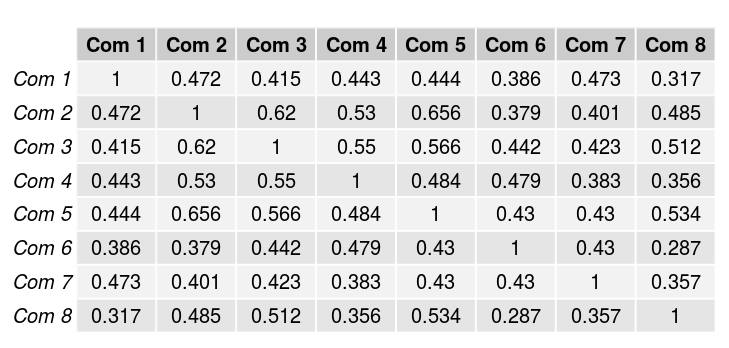
\includegraphics[scale=0.4]{wang_01.png}
			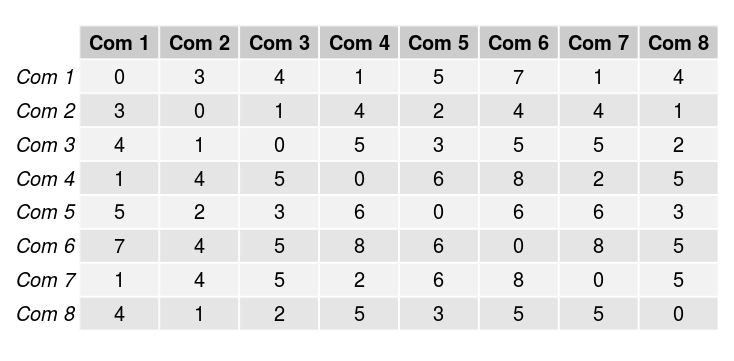
\includegraphics[scale=0.4]{shortest_path_01.png}
			\caption{Example results obtained with the \cite{wang2007new} similarity measurement. 51 communities were found by GHSOM. \textit{Left:} similarities of first 8 communities. \textit{Right:} shortest path length of first 8 communities on map.}
		\end{figure}
		
	\end{frame}	
	
	\begin{frame}{One Possible Explanation}
		\begin{figure}
			\centering
			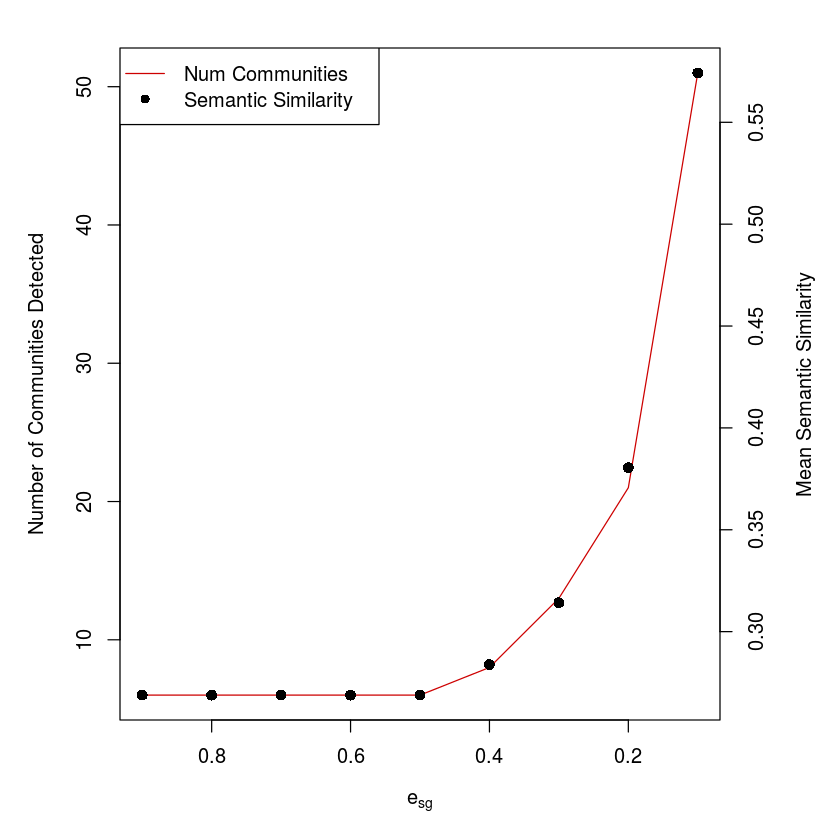
\includegraphics[scale=0.35]{justification.png}
			\caption{Plot of $e_{sg}$ against the number of communities detected in the Uetz screen network and the mean functional similarities of genes in the same community.}
		\end{figure}
	\end{frame}
	
	\begin{frame}{Plans to Finish}
		\begin{itemize}
			\item Search for much smaller communities -- that maximise the functional similarities of clusters.
			\begin{itemize}
				\item Running right now...
			\end{itemize}
			\item Try another type of network: Social networks 
			\begin{itemize}
				\item I have partitioned the Florentine families network and just need ot analyse the results against the ground truths found by other papers.
			\end{itemize}
			\item Compare with results of hierarchical clustering.
			\item Can embedding based on functional similarity rather than shortest path distance produce better results?
		\end{itemize}
	\end{frame}	
	
	\begin{frame}[allowframebreaks]{References}
		\bibliography{references}
		\bibliographystyle{named}
	\end{frame}
	
\end{document}